\chapter{The \PROSE Framework}
\label{ch:prose}

In this section, I describe the methodology of program synthesis the \PROSE framework: \emph{deductive synthesis
driven by domain-specific witness functions}.
I first introduce the notion of witness functions informally in \Cref{sec:prose:intuition}, deriving it from various
instances of prior work in PBE (such as FlashFill and FlashExtract).
Then, in \Cref{sec:prose:wf}, I give a formal definition of witness functions, as well as a comprehensive review of
their usage in PROSE-based PBE technologies.
\Cref{sec:prose:algorithm} presents the main synthesis algorithm of PROSE, \emph{deductive search}.\footnote{Also known
    in the literature as \emph{divide-and-conquer search}, \emph{top-down search}, and \emph{backpropagation-based
    search} (not to be confused with the backpropagation algorithm for training neural
    networks~\cite{chauvin1995backpropagation}, although this name was inspired by similarities between the two
techniques).}
In \Cref{sec:prose:evaluation}, I show its evaluation on $12$+ real-life case studies -- PBE technologies developed on top
of the framework.
Finally, \Cref{sec:prose:discussion} discusses various limitations and extensions to the algorithm.

\section{Intuition}
\label{sec:prose:intuition}
\todoinline{Wrap all big figures in \texttt{\textbackslash begin\{fullpage\}}.}
\todoinline{Mark all \textbf{(a)}, \textbf{(b)}, \dots\ as subfigures with hyperlinks.}

\begin{figure}[p!]
    \begin{fullpage}
        \centering
        \uwsinglespace
        \small
        \hfill\textbf{(a)}
        \vspace{-0.8\baselineskip}
        \begin{algorithmic}
            \Function{GenerateSubstring}{$\sigma$: Input state, $s$: String}
            \State $result \gets \emptyset$
            \ForAll{\hlc{ $(i, k)$ s.t. $s$ is substring of $\sigma(v_i)$ at position $k$ }}
            \State $Y_1 \gets$ \Call{GeneratePosition}{\hlc{$\sigma(v_i), k$}}
            \State $Y_1 \gets$ \Call{GeneratePosition}{\hlc{$\sigma(v_i), k + \mathsf{Length}(s)$}}
            \State $result \gets result \cup \left\{\mathtt{SubStr}(v_i, Y_1, Y_2)\right\}$
            \EndFor
            \State \Return $result$
            \EndFunction

            \Function{GeneratePosition}{$s$: String, $k$: int}
            \State $result \gets \left\{\mathtt{CPos}(\hlc{$k$}), \mathtt{CPos}(\hlc{$-(\mathsf{Length}(s)-k)$})\right\}$
            \ForAll{\hlc{$r_1 = \mathtt{TokenSeq}(T_1, \dots, T_n)$ matching $s[k_1 : k-1]$ for some $k_1$}}
            \ForAll{\hlc{$r_2 = \mathtt{TokenSeq}(T'_1, \dots, T'_m)$ matching $s[k : k_2]$ for some $k_2$}}
            \State \hlc{$r_{12} \gets \mathtt{TokenSeq}(T_1, \dots, T_n, T'_1, \dots, T'_m)$}
            \State \hlc{Let $c$ be s.t. $s[k_1 : k_2]$ is the $c^{\text{th}}$ match for $r_{12}$ in $s$}
            \State \hlc{Let $c'$ be the total number of matches for $r_{12}$ in $s$}
            \State $\tilde{r_1} \gets$ \Call{GenerateRegex}{$r_1, s$}
            \State $\tilde{r_2} \gets$ \Call{GenerateRegex}{$r_2, s$}
            \State $result \gets result \cup \left\{\mathtt{Pos}(\tilde{r_1}, \tilde{r_2}, \left\{\hlc{$c$}, \hlc{$-(c'-c+1)$}\right\})\right\}$
            \EndFor
            \EndFor
            \State \Return $result$
            \EndFunction
        \end{algorithmic}
        \vspace{5pt}
        \hrule
        \vspace{3pt}\hfill\textbf{(b)}
        \vspace{-0.9\baselineskip}
        \begin{algorithmic}
            \Function{Map.Learn}{Examples $\spec$: $\mathsf{Dict}\langle \mathsf{State}, \mathsf{List}\langle T\rangle\rangle$}
            \State Let $\spec$ be $\left\{\state_1 \mapsto Y_1, \dots, \state_m \mapsto Y_m\right\}$
            \For{$j \gets 1\dots m$}
            \State Witness subsequence \hlc{$Z_j \gets \mathsf{Map.Decompose}(\state_j, Y_j)$}
            \EndFor
            \State $\spec_1 \gets$ \hlc{$\bigl\{\state[Z_j[i] / x] \mapsto Y_j[i] \mid i = 0..|Z_j|-1,\, j = 1..m\bigr\}$}
            \State $\vsa_1 \gets F.\mathsf{Learn}(\spec_1)$
            \State $\spec_2 \gets$ \hlc{$\left\{\state_j \mapsto Z_j \mid j = 1..m\right\}$}
            \State $\vsa_2 \gets S.\mathsf{Learn}(\spec_2)$
            \State \Return $\mathsf{Map}(\vsa_1, \vsa_2)$
            \EndFunction
            \\
            \Function{Filter.Learn}{Examples $\spec$: $\mathsf{Dict}\langle \mathsf{State}, \mathsf{List}\langle T\rangle\rangle$}
            \State $\vsa_1 \gets S.\mathsf{Learn}(\hlc{$\spec$})$
            \State $\spec' \gets$ \hlc{$\bigl\{ \state[Y[i]/x] \mapsto \mathsf{true} \mid (\state, Y) \in \spec,\, i = 0..|Y|-1\bigr\}$}
            \State $\vsa_2 \gets F.\mathsf{Learn}(\spec')$
            \State \Return $\mathsf{Filter}(\vsa_2, \vsa_1)$
            \EndFunction
        \end{algorithmic}
        \vspace{3pt}
        \caption{\textbf{(a)} FlashFill synthesis algorithm for learning substring expressions \cite[Figure 7]{flashfill};
            \textbf{(b)} FlashExtract synthesis algorithm for learning $\mathsf{Map}$ and $\mathsf{Filter}$ sequence
            expressions \cite[Figure 6]{flashextract}.
            Highlighted portions correspond to domain-specific computations, which deduce I/O examples for propagation in
            the DSL by ``inverting'' the semantics of the corresponding DSL operator.
        Non-highlighted portions correspond to the search organization, isomorphic between FlashFill and FlashExtract.}
        \label{fig:prose:prior}
    \end{fullpage}
\end{figure}

The main observation behind PROSE is that most of prior synthesis algorithms in PBE can be decomposed into
\begin{enumerate*}[label=\textbf{(\alph*)}]
    \item domain-specific insights for refining a spec for the operator into the specs for its
        parameters, and
    \item a common deductive search algorithm, which leverages these insights for iterative reduction of the synthesis
        problem
\end{enumerate*}.

For instance, \Cref{fig:prose:prior} shows a portion of the synthesis algorithms for FlashFill \cite[Figure
7]{flashfill} and FlashExtract~\cite[Figure 6]{flashextract}.
Both algorithms use a divide-and-conquer approach, reducing a synthesis problem for an expression into smaller synthesis
problems for its subexpressions.
They alternate between three phases, implicitly hidden in the ``fused'' original presentation:
\begin{enumerate}[nosep]
    \item Given some examples for a nonterminal $N$, invoke synthesis on all RHS rules of $N$, and unite the results.
    \item \emph{Deduce} examples that should be propagated to some argument $N_j$ of a current rule $N := F(N_1, \dots,
        N_k)$.
    \item Invoke learning recursively on the deduced examples, and proceed to phase 2 for the subsequent arguments.
\end{enumerate}
Note that phases 1 and 3 do not exploit the \emph{semantics} of the DSL, they only process its \emph{structure}.
In contrast, phase 2 uses domain-specific knowledge to deduce propagated examples for $N_j$ from the examples for $N$.
In \Cref{fig:prose:prior}, we highlight parts of the code that implement phase 2.

It is important that phases 2 and 3 interleave as nested loops for each argument $N_j$ of the currently synthesized
rule, because the examples deduced for an argument $N_{j}$ may depend on the possible value of the
previously processed argument $N_{j-1}$.
For instance, the example positions $k$, deduced for the nonterminal $p$ in \textsc{GenerateSubstring}, depend on the
currently selected possible input string $v_i$.

In FlashExtract, list processing operators $\mathsf{Map}(F, S)$ and $\mathsf{Filter}(F, S)$ are learned generically from
a similar \emph{subsequence spec} $\spec$ of type $\{ \state \tospec \textbf{?} \sqsupseteq
\mathsf{List}\langle T\rangle \}$.
Their learning algorithms are also shown in \Cref{fig:prose:prior}.
Similarly, they are organized in the ``divide-and-conquer'' manner, wherein the given spec is first transformed
into the corresponding parameter specs, and then the synthesis on them is invoked recursively.
FlashExtract provides generic synthesis for five such list\hyp{}processing operators independently of their DSL
instantiations.
However, the domain-specific insight required to build a spec for the $\mathsf{Map}$'s $F$ parameter depends on
the specific DSL instantiation of this $\mathsf{Map}$ (such as $\mathsf{LinesMap}$ or $\mathsf{StartSeqMap}$ in
$\fedsl$), and cannot be implemented in a domain-independent manner.
This insight was originally called a \emph{witness function} -- it \emph{witnessed} sequence elements passed to $F$.
We notice, however, that FlashExtract witness functions are just instances of domain-specific knowledge that
appears in phase~2 of the common meta-algorithm for inductive synthesis.

\subsection{Derivation}
Consider the operator $\mathsf{LinesMap}(F, L)$ in $\fedsl$ (see \Cref{fig:dsl:flashfill}).
It takes as input a \mbox{(sub-)sequence} of lines $L$ in the document, and applies a function $F$ on each line in $L$,
which selects some substring within a given line.
Thus, the simplest type signature of $\mathsf{LinesMap}$ is \mbox{$\left((\mathsf{String} \!\to\!
\mathsf{String}),\, \mathsf{List}\langle\mathsf{String}\rangle\right) \to \mathsf{List}\langle \mathsf{String}
    \rangle$}.

The simplest form of \Cref{problem:syn:general} for $\mathsf{LinesMap}$ is \emph{``Learn all programs of kind
    $\mathsf{LinesMap}(F, L)$ that satisfy a given I/O example $\spec = \state \rightsquigarrow v$''}.
Here $v$ is an output value, i.e. a list of extracted strings.
To solve this problem, we need to compute the following set of expressions:
\begin{equation}
    \left\{\left(F, L\right) \mid \mathsf{LinesMap}(F, L) \models \spec \right\}
    \label{eqn:derivation:problem}
\end{equation}
Applying the principle of divide-and-conquer, in order to solve \eqref{eqn:derivation:problem}, we can compute an
\emph{inverse semantics} of $\mathsf{LinesMap}$:
\begin{equation}
    \mathsf{LinesMap}^{\inv}(v) \bydef \left\{(f, \ell) \mid \mathsf{LinesMap}(f, \ell) = v\right\}
    \label{eqn:derivation:inverse}
\end{equation}
Then, we can recursively learn all programs $F$ and $L$ that evaluate to $f$ and $\ell$ respectively on the input state
$\state$.

\paragraph{Finitization}
Computation of $\mathsf{LinesMap}^{\inv}(v)$ is challenging.
One possible approach could be to enumerate all argument values $f \in \codomain F$, $\ell \in \codomain L$, retaining
only those for which $\mathsf{LinesMap}(f, \ell) = v$.
However, both $\codomain L$ (all string lists) and $\codomain F$ (all $\mathsf{String} \to \mathsf{String}$ functions)
are infinite.\footnote{%
    Here $\codomain F$ denotes the \emph{codomain} of an operator $F$, i.e. the set of its possible outputs.
}

In order to finitize the value space, we apply domain-specific knowledge about the behavior of $\mathsf{LinesMap}$ in
$\fedsl$.
Namely, we use that $L$ must evaluate to a sequence of lines in the input document, and~$F$ must evaluate to a function
that selects a subregion in a given line.
Thus, the ``strongly-typed'' signature of $\mathsf{LinesMap}$ is actually $((\mathsf{Line} \!\to\!
\mathsf{StringRegion}),\,
\mathsf{List}\langle \mathsf{Line}\rangle) \to \mathsf{List}\langle \mathsf{StringRegion}\rangle$
where $\mathsf{StringRegion}$ is a domain-specific type for ``a region within a given document''.
This is a \emph{dependent type}, parameterized by the state $\state$ that contains our input document.
Thus, the inverse semantics $\mathsf{LinesMap}^{\inv}$ is also implicitly parameterized with $\sigma$:
\begin{equation*}
    \mathsf{LinesMap}^{\inv}(\state \rightsquigarrow v) =
    \left\{(f, \ell) \mid
        f \text{ and } \ell \text{ can be obtained from } \state \ \wedge\ \mathsf{LinesMap}(f, \ell) = v
    \right\}
\end{equation*}

Our implementation of $\mathsf{LinesMap}^{\inv}(\state \rightsquigarrow v)$ now enumerates over all line sequences
$\ell$ and substring functions $f$ \emph{given an input document}.
Both codomains are finite.
Note that we took into account both input and output in the spec to produce a constructive synthesis procedure.

\paragraph{Decomposition}
The synthesis procedure above is finite, but not necessarily efficient.
For most values of~$\ell$, there may be no satisfying program $L$ in the DSL to produce it, and therefore even
computing matching values of $f$ for it is redundant.
For instance, let $v = [r_1, r_2]$.
In this case $\ell$ must be the list of two document lines $[l_1, l_2]$ containing $r_1$ and $r_2$, respectively; any
other value for $\ell$ cannot yield $v$ as an output of $\mathsf{LinesMap}(f, \ell)$ regardless of $f$.
In general, \emph{for many domain-specific operators $F(X, Y)$ computing all viable
arguments $(x, y)$ is much slower than computing matching $y$s only for the realizable values of $X$}.

This observation leads to another key idea in PROSE: \emph{decomposition} of inverse semantics.
Namely, for our $\mathsf{LinesMap}$ example, instead of computing $\mathsf{LinesMap}^{\inv}(\state \rightsquigarrow v)$
explicitly, we ask two simpler questions separately:
\begin{enumerate}[nosep]
    \item If $\semantics{\mathsf{LinesMap}(F, L)}{\state} = v$, what could be the possible output of $L$?
    \item If $\semantics{\mathsf{LinesMap}(F, L)}{\state} = v$ and we know that $\semantics{L}{\state} = \ell$, what
        could be the possible output of $F$?
\end{enumerate}
The answers to these questions define, respectively, \emph{partial} and \emph{conditional} inverse semantics of
$\mathsf{LinesMap}$ with respect to its individual parameters:
\begingroup\allowdisplaybreaks
\begin{align}
    \mathsf{LinesMap}^{\inv}_L(v) \ &\supset\ \left\{ \ell \mid \exists f\colon \mathsf{LinesMap}(f, \ell) = v \right\}
    \label{eqn:derivation:inverse} \\
    \mathsf{LinesMap}^{\inv}_F (v \assuming L = \ell) \ &=\ \left\{ f \mid \mathsf{LinesMap}(f, \ell) = v \right\}
    \label{eqn:derivation:conditional}
\end{align}
\endgroup

The key insight of this technique is that, by the principle of \emph{skolemization}~\cite{modeltheory}, inverse
semantics
$\mathsf{LinesMap}^{\inv}(v)$ can be expressed as a cross-product computation of parameter inverses
$\mathsf{LinesMap}^{\inv}_L(v)$ and $\mathsf{LinesMap}^{\inv}_F(v \assuming L = \ell)$ for all possible $\ell \in
\mathsf{LinesMap}^{\inv}_L(v)$:
\begin{gather}
    \begin{aligned}
        \mathsf{LinesMap}^{\inv}(v) = &\left\{(f, \ell) \mid \mathsf{LinesMap}(f, \ell) = v\right\} \\
        = &\left\{(f, \ell) \mid \ell \in \mathsf{LinesMap}^{\inv}(v), f \in \mathsf{LinesMap}^{\inv}_F(v \assuming L = \ell)\right\}
    \end{aligned}
    \label{eqn:derivation:united}
    \raisetag{2\baselineskip}
\end{gather}
Such a decomposition naturally leads to an efficient synthesis procedure for solving the problem
\mbox{$\mathsf{Learn}(\mathsf{LinesMap}(F, L),\ \state \rightsquigarrow v)$}, based on a divide-and-conquer
algorithmic paradigm:
\begin{enumerate}[nosep]
    \item Enumerate  $\ell \in \mathsf{LinesMap}_L^\inv (v)$.
    \item For each $\ell$ recursively find a set of programs $\vsa_{\ell}$ rooted at $L$ such that
        $\semantics{L}{\state} = \ell$.
    \item Enumerate  $f \in \mathsf{LinesMap}_F^\inv (v \assuming L = \ell)$ for all those $\ell$ for which the program
        set $\vsa_{\ell}$ is non-empty.
    \item For each $f$ recursively find a set of programs $\vsa_{\ell,f}$ rooted at $F$ such that $\semantics{F}{\state}
        = f$.
    \item Now, for any such combination of parameter programs $L \in \vsa_{\ell}$, $F \in \vsa_{\ell,f}$ we guarantee
        \mbox{$\mathsf{LinesMap}(F, L) \models \spec$} by construction.
\end{enumerate}

\paragraph{Generalization}
In practice, \Cref{problem:syn:general} for $\mathsf{LinesMap}$ is rarely solved for example-based specs: as
discussed in \Cref{sec:background:spec}, providing the entire output $v$ of regions selected by $\mathsf{LinesMap}$ is
impractical for end users.
Thus, instead of concrete outputs the procedure above should manipulate \emph{specs with properties
    of concrete outputs} (e.g.  a prefix of the output list $v$ instead of entire $v$).
A corresponding generalization of ``inverse semantics of $\mathsf{LinesMap}$'' is a function that deduces a
spec for $L$ given a spec $\spec$ on $\mathsf{LinesMap}(F,\,L)$ (or for $F$, under the assumption of fixed $L$).
We call such a generalization a \emph{witness function}.

In our $\mathsf{LinesMap}$ example, a user might provide a \emph{prefix specification} \mbox{$\spec = \{ \state
\tospec [r_1, r_2, \dots] \}$} for the output list of regions.
The witness functions for such a spec arise naturally:
\begin{itemize}
    \item A witness function for $L$ in this case follows the same observation above: the output list of $L$ should
        begin with two lines containing $r_1$ and $r_2$.
        This is also a prefix specification.
    \item A witness function for $F$ (conditional on $\ell$, the output value of $L$) is universal for all
        $\mathsf{Map}$s: it requires the output of $F$ to be a function that maps the $i^{\text{th}}$ element of $\ell$
        into the $i^{\text{th}}$ element of $[r_1, r_2]$.
        Such modularity of synthesis (a common witness function for any domain-specific $\mathsf{Map}$ operator) is
        another advantage of decomposing inverse semantics into partial and conditional witness functions.
\end{itemize}


\section{Witness Functions}
\label{sec:prose:wf}
As described above, a \emph{witness function} is a generalization of inverse semantics for an operator.
In other words, it is a \emph{problem reduction logic}, which deduces a necessary (or sufficient) spec on the operator's
parameters given a desired spec on the operator's output.
In this section, I define witness functions formally and give various examples of their usages in the existing PBE
technologies.

\begin{defn}[Witness function]
    Let $F(N_1,\dots,N_k)$ be an operator in a DSL $\dsl$.
    A \emph{witness function} of $F$ for $N_j$ is a function $\omega_{j}(\spec)$ that deduces a \emph{necessary}
    spec $\spec_j$ on $N_j$ given a spec $\spec$ on $F(N_1, \dots, N_k)$.
    Formally, $\omega_j(\spec) = \spec_j$ iff $\left[F(N_1, \dots, N_k) \models \spec\right] \wf{} \left[N_j \models
    \spec_j\right]$.\footnote{All free variables are universally quantified unless otherwise specified.}
\end{defn}

\begin{defn}[Precise witness function]
    A witness function $\omega_j$ of $F(N_1, \dots, N_k)$ for $N_j$ is \emph{precise} if its deduced spec is
    \emph{necessary and sufficient}.
    Formally, $\omega_j(\spec) = \spec_j$ is precise iff
    $\left[N_j \models \spec_j\right] \wfc{} \left[\exists\, N_1, \dots, N_{j-1}, N_{j+1}, \dots, N_k\colon\allowbreak
        F(N_1, \dots, N_k) \models \spec \right]$.
\end{defn}

\begin{defn}[Conditional witness function]
    A \emph{(precise) conditional witness function} of $F(N_1, \dots, N_k)$ for $N_j$ is a function $\omega_j(\spec
    \assuming N_{k_1} = v_1, \dots, N_{k_s} = v_s)$ that deduces a necessary (and sufficient) spec $\spec_j$ on $N_j$
    given a spec $\spec$ on $F(N_1, \dots, N_k)$ under the assumption that a subset of other
    parameters $N_{k_1}, \dots, N_{k_s}$ of $F$ (called \emph{prerequisites}) have fixed values $v_1, \dots, v_k$.
    Formally, $\omega_j(\spec \assuming N_t = v_t) = \spec_j$ iff $\left[F(N_1, \dots, N_{t-1}, v_t, N_{t+1}, \dots,
    N_k) \models \spec\right] \wf{} \left[N_j \models \spec_j\right]$.
\end{defn}

\begin{sidewaystable}[p!]
    \begin{fullpage}
        \centering
        % \uwsinglespace
        \small
        \begin{tabu}{lX[-1$l]X[-1$l]X[-1$l]>{\hspace*{1.2em}}X[-3$l]}
            \toprule
            \textbf{Operator} & \textbf{Input spec} & \textbf{Parameter} & \textbf{Prerequisites} & \textbf{Output
            spec} \\
            \midrule
            \dslinline|Concat($atom$,\ $transform$)| & \state \tospec w & atom & &
                \state \tospec \bigvee\limits_{j=1}^{|w|-1} w[0..j] \\
                \cmidrule{3-5}
                & & transform & atom = v & \state \tospec w[|v|..] \\
            \midrule
            \dslinline|ConstStr($s$)| & \state \tospec w & s & & \state \tospec w \\
            \midrule
            \dslinline|let\ $x\ $ = $\ \tikzmark{mark:b:Bind}$std.Kth($inputs$,\ $k$)$\tikzmark{mark:e:Bind}$| &
              \state \tospec w & binding & &
              \state \tospec \bigvee\limits_{\mathclap{j\colon w \text{ occurs in } v_j}}\ v_j \\[3pt]
              \cmidrule{3-5}
          \qquad\dslinline|in Substring($x$,\ $pp$)| & & pp & x = v & \state \tospec
              \bigvee\limits_{\mathclap{\substack{w \text{ occurs in } v \\ \text{ at position } l\ \ }}}
              \ \langle l, l + |w|\rangle \\
            \midrule
            \dslinline|AbsPos($x$,\ $k$)| & \state \tospec c & k & x = v & \state \tospec c \vee c - |v| - 1 \\
            \midrule
            \dslinline|RegexPos($x$, $\ \tikzmark{mark:b:RR}$std.Pair($r$,\ $r$)$\tikzmark{mark:e:RR}$,\ $k$)| &
              \state \tospec c & rr & x = v &
              \state \tospec \bigvee\limits_{\mathclap{\substack{
                          \langle r_1, r_2 \rangle\colon r_1 \text{ matches left of } c \\
                          \hspace*{2.5em}\wedge\ r_2 \text{ matches right of } c}}}\ \langle r_1, r_2 \rangle \\
              \cmidrule{3-5}
              & & k & \begin{aligned} &x = v,\\[0pt] &rr = \langle r_1, r_2 \rangle \end{aligned} &
                  \begin{aligned}
                      &\state \tospec j \vee j - |\vec{c}| - 1 \quad\text{ where } \\
                      &\quad \vec{c} \text{ are the matches of } \langle r_1, r_2 \rangle \text{ in } v, \\
                      &\quad j \text{ is an index of } c \text{ in } \vec{c}
                  \end{aligned} \\
            \bottomrule
        \end{tabu}
        \begin{tikzpicture}[overlay, remember picture]
            \draw[decorate, decoration={brace, mirror}, transform canvas={yshift=-0.3em}]
                (pic cs:mark:b:Bind) -- (pic cs:mark:e:Bind) node[midway, below] {$binding$};
        \end{tikzpicture}
        \begin{tikzpicture}[overlay, remember picture]
            \draw[decorate, decoration={brace, mirror}, transform canvas={yshift=-0.3em}]
                (pic cs:mark:b:RR) -- (pic cs:mark:e:RR) node[midway, below] {$rr$};
        \end{tikzpicture}
        \caption{Witness functions for various FlashFill operators.}
        \label{tbl:wfs:flashfill}
    \end{fullpage}
\end{sidewaystable}

\begin{sidewaystable}[p!]
    \begin{fullpage}
        \centering
        % \uwsinglespace
        \small
        \begin{tabu}{lX[-1$l]X[-1$l]X[-1$l]X[-3$l]}
            \toprule
            \textbf{Operator} & \textbf{Input spec} & \textbf{Parameter} & \textbf{Prerequisites} & \textbf{Output
            spec} \\
            \midrule
            \dslinline|Kth($xs$,\ $k$)| & \state \tospec w & xs & & \state \tospec [\dots, w, \dots] \\
            \cmidrule{3-5}
            & & k & xs = \vec{v} & \state \tospec \bigvee\limits_{v_j = w} j \\
            \midrule
            \dslinline|Pair(|$p_1$\dslinline|,\ |$p_2$\dslinline|)| & \state \tospec \langle v_1, v_2 \rangle & p_j & &
                \state \tospec v_j \\
            \midrule
            \dslinline|Map($F$,\ $L$)| & \state \tospec \mathbf{?} \sqsupseteq \vec{\ell} \text{ as a prefix } & F &
                L = \vec{v} & \state \tospec f \text{ s.t. } \bigwedge\limits_{i=1}^{|\vec{\ell}|} f(v_i) = \ell_i \\
            \midrule
            $\fun{x}\ b$ & \state \tospec f \text{ s.t. } f(v) = y & b & & \state[x \coloneq v] \tospec y \\
            \midrule
            \dslinline|Filter($P$,\ $L$)| & \state \tospec \mathbf{?} \sqsupseteq \vec{\ell} & L & &
                \state \tospec \mathbf{?} \sqsupseteq \vec{\ell} \\
            \cmidrule{3-5}
            & & P & L = \vec{v} & \state \tospec f \text{ s.t. }
                \bigwedge\limits_{i=1}^{|\vec{v}|} f(\ell_i) = \bigl[v_i \in \vec{\ell}\bigr] \\
            \midrule
            \dslinline|FilterInt($i$,\ $k$,\ $L$)| & \state \tospec \mathbf{?} \sqsupseteq \vec{\ell} & L & &
                \state \tospec \mathbf{?} \sqsupseteq \vec{\ell} \\
            \cmidrule{3-5}
            & & i & L = \vec{v} & \state \tospec \text{ index of } \ell_1 \text{ in } \vec{v} \\
            \cmidrule{3-5}
            & & k & L = \vec{v} &
                \begin{aligned}
                    &\state \tospec \bigvee\limits_{d\;|\; g} d \quad\text{ where } \\
                    &\quad g = \mathsf{gcd}\bigl(\Delta_1, \dots, \Delta_{|\vec{\ell}|-1}\bigr), \\
                    &\quad \Delta_i = p_{i+1} - p_i, \\
                    &\quad p_j \text{ is an index of } \ell_j \text{ in } \vec{v}
                \end{aligned} \\
            \bottomrule
        \end{tabu}
        \caption{Witness functions for various operators from the standard library of PROSE (\dslinline|std|).}
        \label{tbl:wfs:prose}
    \end{fullpage}
\end{sidewaystable}



\begin{example}
    \Cref{tbl:wfs:flashfill} shows witness functions for all FlashFill operators from \Cref{fig:dsl:flashfill}:
    \begin{itemize}[nosep]
        \item A \dslinline|Concat($atom$, $transform$)| expression returns $w$ iff $atom$ returns some prefix of $w$.
            In addition, assuming that $atom$ returns $v$, $transform$ mush return the remaining suffix of~$w$ after the
            end of $v$.
        \item A \dslinline|ConstStr($s$)| expression returns $w$ iff $s$ is equal to $w$.
        \item An expression ``\dslinline|let $x$ = std.Kth($inputs$, $k$) in $\dots$|'' returns $w$ iff $x$ is bound to
            an element of $inputs$ that has $w$ as a substring.
        \item A \dslinline|Substring($x$, $pp$)| expression returns $w$ (assuming that $x$ returns $v$) iff $pp$ returns
            a position span of any occurrence of $w$ in $v$ as a substring.
        \item An \dslinline|AbsPos($x$, $k$)| expression returns $c$ (assuming that $x$ returns $v$) iff $k$ is equal to
            either~$c$ or $c-|v|-1$ (since $k$ may represent a left or right offset depending on its sign).
        \item An expression \dslinline|RegexPos($x$, $rr$, $k$)| returns $c$ (assuming that $x$ returns $v$) iff $rr$ is
            equal to any pair of regular expressions that matches the boundaries of position $c$ in the string~$v$.
            In addition, assuming that $rr$ is equal to $\langle r_1, r_2\rangle$, $P$ returns $c$ iff $k$ is equal to
            a index of $c$ (from the left or right) among all matches of $\langle r_1, r_2\rangle$ in $v$.
    \end{itemize}
    \label{ex:wf:flashfill}
\end{example}

Most witness functions are domain-specific w.r.t.  the operator that they characterize.
However, once formulated in a module for a domain such as substring extraction, they can be reused by any DSL.
In our example, witness functions for $\mathsf{Pair}$ and $\mathsf{Kth}$ operators in \Cref{tbl:wfs:prose} do not
depend on the domain of their parameters, and are therefore formulated generically, for any DSL.
Witness functions in \Cref{tbl:wfs:flashfill} hold only for their respective operators, but they do
not depend on the rest of the DSL in which these operators are used, provided the operator semantics is conformant with
its (strongly-typed) signature.
This property allows us to define witness functions as generally as possible in order to reuse the corresponding
operators in any conformant DSL.

\section{Deductive Search}
\label{sec:prose:algorithm}

A set of witness functions for all the parameters of an operator allows us to reduce the inductive synthesis problem
$\langle N, \spec\rangle$ to the synthesis subproblems for its parameters.
We introduce a simple non-conditional case first, and then proceed to complete presentation of the entire algorithm.

\begin{theorem}
    Let $N := F(N_1, \dots, N_k)$ be a rule in a DSL $\dsl$, and $\spec$ be a spec on $N$.
    Assume that $F$ has $k$ non-conditional witness functions $\omega_j(\spec) = \spec_j$,
    and $\vsa_j \models \spec_j$ for all $j = 1..k$ respectively.
    \begin{enumerate}[nosep]
        \item $\mathsf{Filter}(\joinCons(\vsa_1, \dots, \vsa_k), \spec) \models \spec$.
        \item If all $\omega_j$ are precise, then $\joinCons(\vsa_1, \dots, \vsa_k) \models \spec$.
    \end{enumerate}
    \label{thm:wf:noncond}
\end{theorem}
\begin{proof} \leavevmode
    \begin{enumerate}[nosep]
        \item By definition of $\mathsf{Filter}(\vsa, \spec)$.
        \item All $\omega_j$ deduce specs for $N_j$ given only the outer spec $\spec$, therefore they
            are independent from each other.
            Also, all $\omega_j$ are precise, therefore each $\vsa_j$ individually is necessary and sufficient to
            satisfy $\spec$. \qedhere
    \end{enumerate}
\end{proof}

\Cref{thm:wf:noncond} gives a straightforward recipe for synthesis of operators with independent parameters, such as
\dslinline|Pair($p_1$, $p_2$)|.
However, in most real-life cases operator parameters are dependent on each other.
Consider an operator \dslinline|Concat($atom$, $transform$)| from FlashFill, and a spec $\state \tospec s$.
It is possible to design individual witness functions $\omega_a$ and $\omega_t$ that return a disjunction $\spec_a$ of
prefixes of $s$ and a disjunction $\spec_t$ of suffixes of $s$, respectively.
Both of these witness functions individually are precise (i.e. sound and complete); however, there is no straightforward
way to combine recursive synthesis results $\vsa_a \models \spec_a$ and $\vsa_t \models \spec_t$ into a valid program
set for $\spec$.

In order to enable deductive search for dependent operator parameters, we apply \emph{skolemization}~\cite{modeltheory}.
Instead of deducing specs $\spec_a$ and $\spec_t$ that independently entail $\spec$, we deduce only one
independent spec (say, $\spec_a$), and then \emph{fix the value of ``$atom$''}.
For each fixed value of $atom$ a \emph{conditional witness function} $\omega_t(\spec \assuming atom = v)$ deduces a
spec $\spec_{t,v}$ that is a necessary and sufficient characterization for $\spec$.
Namely, $\spec_{t,v}$ in our example is $\state \tospec s[|v|..]$ (i.e. the remaining suffix) if $v$ is a prefix of~$s$,
or $\bot$ otherwise.

Skolemization splits the deduction into multiple independent branches, one per each value of $atom$.
These values are determined by VSA clustering: \mbox{$\clustering[\vsa_a] = \{v_1 \mapsto \vsa_a^1,
\dots, v_k \mapsto \vsa_a^k\}$}.
Within each branch, the program sets $\vsa_a^j$ and the corresponding $\vsa_t^j \models \spec_{t,v_j}$ are
independent, hence $\joinCons[\mathsf{Concat}](\vsa_a^j, \vsa_t^j) \models \spec$ by \Cref{thm:wf:noncond}.
The union of $k$ branch results constitutes a comprehensive set of all $\mathsf{Concat}$ programs that satisfy $\spec$.

\begin{defn}
    Let $N := F(N_1, \dots, N_k)$ be a rule in a DSL $\dsl$ with $k$ associated (possibly conditional) witness functions
    $\omega_1, \dots, \omega_k$.
    A \emph{dependency graph} of witness functions of $F$ is a directed graph $G(F) = \langle V, E\rangle$ where $V=
    \left\{N_1, \dots, N_k\right\}$, and $\langle N_i, N_j\rangle \in E$ iff $N_i$ is a prerequisite for $N_j$.
\end{defn}

A dependency graph can be thought of as a union of all possible Bayesian networks over parameters of $F$.
It is not a single Bayesian network because $G(F)$ may contain cycles: it is often possible to independently express
$N_i$ in terms
of $N_j$ as a witness function $w_i(\spec \assuming N_j = v)$ and $N_j$ in terms of $N_i$ as a different witness
function $w_j(\spec \assuming N_i = v)$.
One simple example of such phenomenon is \dslinline|Concat($atom$, $transform$)|: we showed above how to decompose its
inverse semantics into a witness function for prefixes and a conditional witness function for the suffix, but a
symmetrical decomposition into a witness function for suffixes and a conditional witness function for prefixes is also
possible.

\begin{figure}[p!]
    \begin{fullpage}
        \small
        \uwsinglespace
        \begin{algorithmic}[1]
            \Given{G(F)}{dependency graph of witness functions for the rule $F$}
            \Given{\spec}{specification for the rule $F$}
            \Functionx{LearnRule}{$G(F), \spec$}
            \State Permutation $\pi \gets \mathsf{TopologicalSort}(G(F))$
            \State $\vsa \gets \bigvsaunion \bigl\{ \vsa' \bigmid \vsa' \in \Call{LearnPaths}{G(F), \spec, \pi, 1, \varnothing} \bigr\}$
            \If{all witness functions in $G(F)$ are precise}
            \State \Return $\vsa$
            \Else
            \State \Return $\mathsf{Filter}(\vsa, \spec)$
            \EndIf
            \EndFunction
            \Statex
            \Given{\pi}{permutation of the parameters of $F$}
            \Given{i}{index of a current deduced parameter in $\pi$}
            \Given{Q}{a mapping of prerequisite values $\values_{k}$ and corresponding learnt program sets $\vsa_{k}$ on the current path}
            \Functionx{LearnPaths}{$G(F), \spec, \pi, i, Q$}
            \If{$i > k$}
            \State Let $\vsa_1, \dots, \vsa_k$ be learnt program sets for $N_1, \dots, N_k$ in $Q$
            \State \Return $\left\{ \joinCons(\vsa_1, \dots, \vsa_k) \right\}$
            \EndIf
            \State $p \gets \pi_i$ \Comment{Current iteration deduces the rule parameter $N_p$}
            \State Let $\omega_{p}(\spec \assuming N_{k_1} = \values_1, \dots, N_{k_m} = \values_m)$ be the witness
            function for $N_{p}$
            \Statex \Comment{Extract the prerequisite values for $N_{p}$ from the mapping $Q$}
            \State $\{\values_{k_1} \mapsto \vsa_{k_1}, \dots, \values_{k_m} \mapsto \vsa_{k_m}\} \gets Q[k_1, \dots, k_m]$
            \Statex \Comment{Deduce the spec for $N_{p}$ given $\spec$ and the prerequisites}
            \State $\spec_{p} \gets \omega_{p}(\spec \assuming N_{k_1} = \values_{k_1}, \dots, N_{k_m} = \values_{k_m})$ \label{alg:line:wf}
            \If{$\omega_p = \bot$}
            \Return $\emptyset$
            \EndIf
            \Statex \Comment{Recursively learn a valid program set $\vsa_{p} \models \spec_{p}$}
            \State $\vsa_{p} \gets \mathsf{Learn}(N_{p}, \spec_{p})$ \label{alg:line:sublearn}
            \Statex \Comment{If no other parameters depend on $N_{p}$, proceed without clustering}
            \If{$N_{p}$ is a leaf in $G(F)$}
            \State $Q' \gets Q[p := \top \mapsto \vsa_{p}]$
            \State \Return \Call{LearnPaths}{$G(F), \spec, \pi, i+1, Q'$}
            \Statex \Comment{Otherwise cluster $\vsa_{p}$ on $\states$ and unite the results across branches}
            \Else
            \State $\states \gets$ the input states associated with $\spec$
            \ForAll{$\bigl(\values'_j \mapsto \vsa'_{s,j}\bigr) \in \clustering[\vsa_p][\states]$} \label{alg:line:clusters}
            \State $Q' \gets Q\bigl[s := \values'_j \mapsto \vsa'_{s,j}\bigr]$
            \State \Yield \textbf{all} \Call{LearnPaths}{$G(F), \spec, \pi, i+1, Q'$}
            \EndFor
            \EndIf
            \EndFunction
        \end{algorithmic}
        % \end{mdframed}
        \caption{A learning procedure for the DSL rule $N := F(N_1, \dots, N_k)$ that uses $k$ conditional witness functions
        for $N_1, \dots, N_k$, expressed as a dependency graph $G(F)$.}
        \label{fig:prose:algorithm}
    \end{fullpage}
\end{figure}

\begin{theorem}
    Let $N := F(N_1, \dots, N_k)$ be a rule in a DSL $\dsl$, and $\spec$ be a spec on $N$.
    If there exists an acyclic spanning subgraph of $G(F)$ that includes each node with all its prerequisite edges, then
    there exists a polynomial procedure that constructs a valid program set $\vsa \models \spec$ from the valid
    parameter program sets $\vsa_j \models \spec_j$ for some choice of parameter specifications $\spec_j$.
    \label{thm:wf:cond}
\end{theorem}
\begin{proof}
    We define the learning procedure for $F$ in \Cref{fig:prose:algorithm} algorithmically.
    It recursively explores the dependency graph $G(F)$ in a topological order, maintaining a \emph{prerequisite path}
    $Q$ -- a set of
    parameters $N_j$ that have already been skolemized, together with their fixed bindings~$\values_j$ and valid program
    sets $\vsa_j$.
    In the prerequisite path, we maintain the invariant: \emph{for each program set $\vsa_j$ in the path, all programs
        in it produce the same values $\values_j$ on the provided input states~$\states$}.
    This allows each conditional witness function $\omega_{i}$ to deduce a spec $\spec_i$ for the current
    parameter~$N_i$ assuming the bound values $\values_{k_1}, \dots, \values_{k_s}$ for the prerequisites
    $N_{k_1}, \dots, N_{k_s}$ of $N_i$.

    The program sets in each path are valid for the subproblems deduced by applying witness functions.
    If all the witness functions in $G(F)$ are precise, then any combination of programs $P_1, \dots, P_k$ from these
    program sets yields a valid program $F(P_1, \dots, P_k)$ for $\spec$.
    If some witness functions are imprecise, then a filtered join of parameter program sets for each path is valid
    for $N$.
    Thus, the procedure in \Cref{fig:prose:algorithm} computes a valid program set $\vsa \models \spec$.
\end{proof}

\Cref{thm:wf:noncond,thm:wf:cond} give a \emph{constructive} definition of the refinement procedure that splits the
search space for $N$ into smaller parameter search spaces for $N_1,\dots,N_k$.
If the corresponding witness functions are precise, then \emph{every} combination of valid parameter programs from these
subspaces yields a valid program for the original synthesis problem.
Alternatively, if some of the accessible witness functions are imprecise, we use them to \emph{narrow down} the
parameter search space, and filter the constructed program set for validity.
The $\mathsf{Filter}$ operation (defined in \Cref{ch:vsa}) filters out inconsistent programs from $\vsa$ in time
proportional to $\clustering$.

\begin{sidewaysfigure}[p!]
    \begin{fullpage}
        \centering
        \def\sAtom{\text{\ttfamily atom}\,}
\def\sTransform{\text{\ttfamily transform}\,}
\hspace*{-6pt}
\begin{tikzpicture}[transform shape, remember picture,
                    deductive/.style={draw=SandyBrown, fill=SandyBrown!65, rounded corners=5pt,
                        align=left, inner sep=10pt},
                    entry/.style={draw=none, align=left},
                    fatarrow/.style={-{Triangle[scale=0.5]}, line width=8pt, draw=LightSkyBlue}]
    \large
    \uwsinglespace
    \tcbset{tile, size=title, on line, boxrule=0pt, colback=LightSkyBlue}
    \node[entry] (n-root) {$\langle \sTransform,\ \spec\rangle$};

    \node[entry, below right=2cm and -2.5cm of n-root] (n-concat)
        {$\langle\mathsf{Concat}\left(\sAtom,\, \sTransform\right),\ \spec\rangle$};
    \node[deductive, below=5pt of n-concat] (ded-concat) {%
        $\begin{aligned}
            &\spec_1 \coloneqq \omega_a\left(\spec\right) \\
            &\vsa_1 \coloneqq \subnode{learn-atom}{\tcbox{$\mathsf{Learn}\left(\sAtom, \spec_1\right)$}} \\
            &\{ o_1 \mapsto \vsa'_1,\, o_2 \mapsto \vsa'_2 \} \coloneqq \clustering[\vsa_1]
        \end{aligned}$};
    \draw[fatarrow] ($(n-root.south west) + (0.5cm,0)$) |- (n-concat.west);

    \node[entry, anchor=north west] at ($(ded-concat.south west) - (0,1.5cm)$) (n-atom)
        {$\langle \sAtom,\, \spec\rangle$};
    \draw[fatarrow] ($(n-root.south west) + (0.5cm,0)$) |- (n-atom.west);
    \node[entry, right=1cm of n-atom] (dots-atom) {$\dots$};
    \draw[fatarrow] (n-atom) -- (dots-atom);

    \node[entry, anchor=south] at ($(n-concat.north east) + (-0.7cm,1cm)$) (n-atom1)
        {$\langle \sAtom,\, \spec_1\rangle$};
    \draw[fatarrow, overlay] ($(learn-atom.east) - (11pt,0)$) -| ($(n-atom1.south east) - (15pt,0)$);

    \node[entry, left=1cm of n-atom1] (dots-atom1) {$\dots$};
    \draw[fatarrow] (n-atom1) -- (dots-atom1);

    \coordinate (c-right) at ($(n-atom1) + (4.5cm,0)$);
    \node[deductive, anchor=south west] at (c-right|-n-atom.south) (ded-cluster2) {%
        $\begin{aligned}
            &\spec_{22} \coloneqq \omega_t\left(\spec \assuming \sAtom = \stringliteral{20}\right) \\
            &\subnode{vsa-learn2}{$\color{Green}\vsa_{22}$} \coloneqq \subnode{learn-transform2}{\tcbox{%
                $\mathsf{Learn}\left(\sTransform,\, \spec_{22}\right)$}}
        \end{aligned}$};
    \draw[fatarrow, rounded corners=5pt, color=SandyBrown!65] ($(ded-concat.south east) - (0.5cm,0)$) |- (ded-cluster2);
    \node[entry, anchor=south east] at ($(ded-cluster2.north east) + (0, 0.6cm)$) (n-transform2)
        {$\langle \sTransform,\, \spec_{22} \rangle$};
    \draw[fatarrow] ($(learn-transform2.north east) - (14.2pt,11pt)$) -- ($(n-transform2.south east) - (13.9pt, -3pt)$);
    \node[entry, left=1cm of n-transform2] (dots-transform2) {$\dots$};
    \draw[fatarrow] (n-transform2) -- (dots-transform2);

    \coordinate(c-branch-x) at ($(n-atom1.south east) + (0.7cm,0)$);
    \coordinate (c-branch) at (c-branch-x|-ded-cluster2);
    \node[deductive, anchor=west] at (c-right|-n-concat.east) (ded-cluster1) {%
        $\begin{aligned}
            &\spec_{21} \coloneqq \omega_t\left(\spec \assuming \sAtom = \stringliteral{2}\right) \\
            &\subnode{vsa-learn1}{$\color{Green}\vsa_{21}$} \coloneqq \subnode{learn-transform1}{\tcbox{%
                $\mathsf{Learn}\left(\sTransform,\, \spec_{21}\right)$}}
        \end{aligned}$};
    \draw[fatarrow, rounded corners=5pt, color=SandyBrown!65] (c-branch) |- (ded-cluster1);
    \node[entry, anchor=south east] at ($(ded-cluster1.north east) + (0, 0.6cm)$) (n-transform1)
        {$\langle \sTransform,\, \spec_{21} \rangle$};
    \draw[fatarrow] ($(learn-transform1.north east) - (14.2pt,11pt)$) -- ($(n-transform1.south east) - (13.9pt, -3pt)$);
    \node[entry, left=1cm of n-transform1] (dots-transform1) {$\dots$};
    \draw[fatarrow] (n-transform1) -- (dots-transform1);

    \coordinate (c-branch-upper) at (c-branch|-ded-cluster1);
    \node[entry, color=Green, above right=0.3cm of c-branch] (n-vsa2) {$\vsa'_2$};
    \node[entry, below right=0.3cm of c-branch] (n-o2) {$o_2 = \stringliteral{20}$};
    \node[entry, color=Green, above right=0.3cm of c-branch-upper] (n-vsa1) {$\vsa'_1$};
    \node[entry, below right=0.3cm of c-branch-upper] (n-o1) {$o_1 = \stringliteral{2}$};

    \begin{scope}[on background layer]
        \node[anchor=north east, outer sep=3pt] at (n-o2.south west) (join2-sw) {};
        \node[above right=0.1cm of n-transform2.north east] (join2-ne) {};
        % \filldraw[color=PaleGreen!40, rounded corners=10pt] (join2-sw) rectangle (join2-ne);
        \node[entry, color=Green, anchor=north west, inner sep=6pt] at (join2-ne-|join2-sw) (join2-concat)
            {$\joinCons[\mathsf{Concat}]$};

        \node[anchor=north east, outer sep=3pt] at (n-o1.south west) (join1-sw) {};
        \node[above right=0.1cm of n-transform1.north east] (join1-ne) {};
        % \filldraw[color=PaleGreen!40, rounded corners=10pt] (join1-sw) rectangle (join1-ne);
        \node[entry, color=Green, anchor=north west, inner sep=6pt] at (join1-ne-|join1-sw) (join1-concat)
            {$\joinCons[\mathsf{Concat}]$};

        \node[entry, node font=\color{Green}, above left=0.2cm of c-branch] (union-inner) {$\bigvsaunion$};
        \node[entry, node font=\color{Green}, below right=0cm and .6cm of n-root.south west]
            (union-outer) {$\bigvsaunion$};
    \end{scope}
    \begin{scope}[every path/.style={-Stealth, dotted, thick, color=Green, rounded corners=10pt}]
        \draw (union-inner.north) |- (join2-concat.west);
        \draw (union-inner.north) |- (join1-concat.west);
        \draw (union-outer.south) |- (union-inner.west);
        \draw ($(join1-concat.south)!0.4!(join1-concat.south west)$) -- (n-vsa1);
        \draw ($(join1-concat.south)!0.5!(join1-concat.south east)$) to[bend left]
            ($(vsa-learn1.center)!0.5!(vsa-learn1.north)$);
        \draw ($(join2-concat.south)!0.4!(join2-concat.south west)$) -- (n-vsa2);
        \draw ($(join2-concat.south)!0.5!(join2-concat.south east)$) to[bend left]
            ($(vsa-learn2.center)!0.5!(vsa-learn2.north)$);
        \draw[sharp corners] (union-inner.west) -| (dots-atom.north);
    \end{scope}
\end{tikzpicture}

        \large
        \vspace*{-\baselineskip}
        \begin{equation*}
            \spec\colon\ \stringliteral{(202) 555-0126} \tospec \stringliteral{202}
            \quad
            \spec_1\colon\ \stringliteral{(202) 555-0126} \tospec \stringliteral{2} \,\vee\, \stringliteral{20}
            \quad
            \begin{aligned}[t]
                &\spec_{21}\colon\ \stringliteral{(202) 555-0126} \tospec \stringliteral{02} \\[-0.3\baselineskip]
                &\spec_{22}\colon\ \stringliteral{(202) 555-0126} \tospec \stringliteral{2}
            \end{aligned}
        \end{equation*}
        \caption{An illustrative diagram showing the outermost layer of deductive search for a given problem
        $\mathsf{Learn}\left(\mathtt{transform}\,,\, \stringliteral{(202) 555-0126} \tospec \stringliteral{202}\right)$.
        Solid blue arrows show the recursive calls of the search process (the search subtrees below the outermost layers
        are not expanded and shown as ``\dots'').
        Rounded orange blocks and arrows shows the nested iterations of the \textsc{LearnPaths} procedure from
        \Cref{fig:prose:algorithm}.
        Dotted green arrows show the VSA structure that is returned to the caller.}
        \label{fig:prose:algorithm:example}
    \end{fullpage}
\end{sidewaysfigure}

\begin{example}
    \Cref{fig:prose:algorithm:example} shows an illustrative diagram for the outermost layer of the learning process for
    the \dslinline|$transform$| symbol from $\ffdsl$ and a given spec $\spec = \stringliteral{(202) 555-0126} \tospec
    \stringliteral{202}$.
    First, the framework splits the search process into two branches: one for \dslinline|Concat($atom$, $transform$)|
    and one for \dslinline|$atom$|, according to the definition of \dslinline|$transform$| in $\ffdsl$.
    The figure shows the outermost layer of the first branch.

    The \textsc{LearnPaths} procedure first invokes the witness function $\omega_a$ for the first
    parameter $atom$ of the \dslinline|Concat| rule.
    It returns a necessary spec $\spec_1 = \state \tospec \stringliteral{2} \,\vee\,
    \stringliteral{20}$ for the $atom$ symbol (where $\state$ is the shared input state from $\spec$).
    The PROSE framework then recursively resolves this spec into a VSA $\vsa_1$ of all $atom$ programs that satisfy
    $\spec_1$.

    Next, the \textsc{LearnPaths} procedure clusters $\vsa_1$ and splits its further execution into two branches, one
    per each cluster of programs in $\vsa_1$ that give the same output on the given input state $\state$.
    There are two clusters: programs $\vsa'_1$ that return $o_1 = \stringliteral{2}$ and programs $\vsa'_2$ that return
    $o_2 = \stringliteral{20}$.
    For each of them the PROSE framework independently invokes a nested call to \textsc{LearnPaths} with the
    corresponding output binding for $atom$ (i.e. $o_1$ or $o_2$ respectively) recorded in the prerequisite path $Q$.
    Within each nested invocation, \textsc{LearnPaths} constructs a necessary and sufficient spec on the second
    parameter $transform$ of \dslinline|Concat| by invoking its conditional witness function $\omega_t$.
    It returns a spec $\spec_{21}\colon\ \state \tospec \stringliteral{02}$ for the branch with $o_1 =
    \stringliteral{2}$ and a spec $\spec_{22}\colon\ \state \tospec \stringliteral{2}$ for the branch with $o_2 =
    \stringliteral{20}$, respectively.
    The framework then recursively resolves them into the corresponding program sets $\vsa_{21}$ and $\vsa_{22}$.

    Since both witness functions $\omega_a$ and $\omega_t$ are precise, the final result returned from
    \textsc{LearnPaths} is the VSA $\vsaunion\left\{ \joinCons[\mathsf{Concat}]\left(\vsa'_1,\, \vsa_{21}\right),\,
    \joinCons[\mathsf{Concat}]\left(\vsa'_2,\, \vsa_{22}\right) \right\}$.
\end{example}

\section{Evaluation}
\label{sec:prose:evaluation}
Our evaluation of PROSE aims to answer two classes of questions: its \emph{applicability} and its \emph{performance}.
Applicability questions concern (a) our generalization of prior work in PBE
in terms of inductive specifications and witness functions; (b) generality of our library of witness functions;
(c) engineering usability of PROSE.
Performance questions concern the running time of synthesizers generated by PROSE, and the comparison of
PROSE to general-purpose non-inductive synthesizers, such as SyGuS~\cite{sygus}.

\subsection{Case Studies}
\label{sec:prose:evaluation:casestudies}
\Cref{tbl:prose:casestudies} summarizes our case studies: the prior works in inductive synthesis over numerous different
applications that we studied for evaluation of PROSE.
Of the \ref*{case:total} inductive synthesis tools we studied, \ref*{case:totaldc} can be cast as a special case of the
deductive search algorithm
methodology, which we verified by manually formulating corresponding witness functions for their algorithms.
In the other \pgfmathparse{int(\getrefnumber{case:total}-\getrefnumber{case:totaldc})}\pgfmathresult~tools, the
application domain is inductive synthesis, and our problem definition covers their application, but the original
technique is not an instance of deductive search: namely, it is enumerative
search~\cite{transit:protocols,magichaskeller} or constraint solving~\cite{quicksilver}.

\begin{table}[p!]
    \centering
    \small
    \newcounter{casenum}
    \setcounter{casenum}{-1}
    \begin{tabular}{>{\refstepcounter{casenum}}llcccc}
        \toprule
        \textbf{Project} & \textbf{Domain} & \textbf{Ded.} & \textbf{Impl.} & $\bm{\constraint}$ & $\bm{\spec'}$ \\
        \midrule
        \citet{flashfill} & String transformation & \yesmark & \yesmark & = & = \\
        \citet{flashextract} & Text extraction &  &  & $\sqsupset$ & $\sqsupset$ \\
        \citet{flashnormalize} & Text normalization &  &  & = & soft \\
        \citet{flashrelate} & Table normalization &  &  & = & = \\
        \label{case:totalreimpl}\citet{singh2012synthesizing} & Number transformation &  &  & = & = \\
        \midrule
        \citet{vldb12:semantic} & Semantic text editing & \yesmark & \nomark & = & = \\
        \citet{harris2011spreadsheet} & Table transformation &  &  & = & = \\
        \citet{andersen:procedural} & Algebra education &  &  & trace & = \\
        \citet{lau:smartedit} & Editor scripting &  &  & trace & = \\
        \citet{pldi15:swarat} & ADT transformation &  &  & = & = \\
        \citet{pldi15:osera} & ADT transformation &  &  & = & = \\
        \label{case:totaldc}\citet{miller:colorful} & Editor scripting &  &  & = & = \\
        \midrule
        \citet{transit:protocols} & Concurrent protocols & \nomark & \nomark & trace & N/A \\
        \citet{magichaskeller} & Haskell programs &  &  & = & N/A \\
        \label{case:total}\citet{quicksilver} & Relational queries &  &  & = & N/A \\
        \midrule
        \citet{raza2017automated} & Splitting of text into columns & \yesmark & \yesmark & = & = \\
        \citet{refazer} & Software refactoring & & & = & = \\
        \citet{gorinova2016end} & Reshaping of healthcare data & & & = & $\approx$ \\
        \textsf{Transformation.JSON} & Transformation of JSON trees &  &  & = & $\sqsupset$ \\
        \textsf{Extraction.JSON} & Extraction of data from JSON files &  &  & $\sqsupset$ & $\sqsupset$ \\
        \textsf{Matching.Text} & Data profiling/clustering &  &  & --- & = \\
        \label{case:totalwithnew}\textsf{Extraction.Web} & Web data extraction &  &  & $\sqsupset$ & $\sqsupset$ \\
        \bottomrule
    \end{tabular}
    \uwsinglespace
    \caption{Case studies of PROSE: prior works in inductive program synthesis.
        ``Ded.'' means ``Is it an instance of the deductive methodology?'',
        ``Impl.'' means ``Have we (re-)implemented it on top of PROSE?'', $\constraint$ is a top-level constraint kind,
        $\spec'$ lists notable intermediate constraint kinds (for the deductive techniques only).
        The bottommost section shows the new projects implemented on top of PROSE since its creation.}
    \label{tbl:prose:casestudies}
\end{table}

\begin{table}[t]
    \centering
    \begin{tabular}{lllll}
        \toprule
        \multicolumn{1}{c}{\multirow{2}{*}{\textbf{Project}}} & \multicolumn{2}{c}{\textbf{LOC}} &
            \multicolumn{2}{c}{\textbf{Development time}} \\
        \cmidrule{2-3}  \cmidrule{4-5}
        & Original & PROSE & Original & PROSE \\
        \midrule
        \citet{flashfill} & 12K & 3K & 9 months & 1 month \\
        \citet{flashextract} & 7K & 4K & 8 months & 1 month \\
        \citet{flashnormalize} & 17K & 2K & 7 months & 2 months \\
        \citet{flashrelate} & 5K & 2K & 8 months & 1 month \\
        \citet{singh2012synthesizing} & --- & 1K & --- & 2 months \\
        \midrule
        \citet{raza2017automated} & --- & 10K & --- & 2 months \\
        \citet{refazer} & & 6K & & 3 months \\
        \textsf{Transformation.JSON} & & 2K & & 1 month \\
        \textsf{Extraction.JSON} & & 3K & & 1 month \\
        \textsf{Matching.Text} & & 2K & & 3 months \\
        \textsf{Extraction.Web} & & 2.5K & & 1.5 months \\
        \bottomrule
    \end{tabular}
    \caption{Development data on the (re-)implemented projects.
        The cells marked with ``---'' either do not have an original implementation or we could not obtain historical
    data on them.}
    \label{tbl:prose:reimplementation}
\end{table}

Our industrial collaborators reimplemented \ref*{case:totalreimpl} existing systems
and created \pgfmathparse{int(\getrefnumber{case:totalwithnew}-\getrefnumber{case:total})}\pgfmathresult~new ones since
PROSE was created in \citeyear{flashmeta}.
We present data on these development efforts in \Cref{tbl:prose:reimplementation}.

\paragraph{Q1: How motivated is our generalization of inductive specification?}
Input-output examples is the most popular specification kind, observed in 12/\ref*{case:total} projects.
However, 3 projects require \emph{program traces} as their top-level specification, and 2 projects (1 prior) require
\emph{subsequences of program output}.
Boolean connectives such as $\vee$ and $\neg$ are omnipresent in subproblems across all \ref*{case:totaldc} projects
implemented using deductive search.

\paragraph{Q2: How applicable is our generic operator library?}
Most common operators across our case studies are string processing functions, due to the most popular domain being data
manipulation (11/\ref*{case:totalwithnew} projects).
Almost all projects include some version of learning conditional operators (equivalent to that of FlashFill).
List processing operators (e.g. $\mathsf{Map}$, $\mathsf{Filter}$) appear in 9/\ref*{case:totalwithnew} projects, often
without explicit realization by the original authors (for example, the awkwardly defined \textsf{Loop} operator in
FlashFill is actually a combination of \textsf{Concatenate} and \textsf{Map}).
\citet{pldi15:swarat} define an extensive library of synthesis strategies for list-processing operators in the
$\lambda^2$ project.
These synthesis strategies are isomorphic to FlashExtract witness functions; both approaches can be cast as instances of
deductive search (see \Cref{ch:related} for detailed comparison).

\paragraph{Q3: How usable is PROSE?}
\Cref{tbl:prose:reimplementation} presents some development stats on the projects that were reimplemented.
In all cases, PROSE-based implementations were shorter, cleaner, more stable and extensible.
The reason is that with PROSE, our collaborators did not concern themselves with tricky details of synthesis
algorithms, since they were implemented once and for all, as in \Cref{sec:prose:algorithm}.
Instead, they focused only on domain-specific witness functions, for which design, implementation, and maintenance are
much easier.
Notably, in case of the FlashRelate~\cite{flashrelate} reimplementation and \textsf{Extraction.Web}, our collaborators
did not have any experience in program synthesis.

The development time in \Cref{tbl:prose:reimplementation} includes the time required for an implementation to mature
(i.e. cover the required use cases), which required multiple experiments with DSLs.
With PROSE, various improvements over DSLs were possible on a daily basis.
PROSE also allowed our collaborators to discover optimizations not present in the original implementations.
We share some anecdotes of PROSE simplifying synthesizer development below.

\begin{scenario}
    One of the main algorithmic insights of FlashFill is synthesis of $\mathsf{Concat}(e_1, \dots, e_k)$ expressions
    using \emph{DAG program sharing}.
    A DAG over the positions in the output string $s$ is maintained, each edge $s[i:j]$ annotated with a
    set of programs that output this substring on a given state $\state$.
    Most of the formalism in the paper and code in their implementation is spent on describing and performing operations
    on such a DAG.
    In PROSE, the same grammar symbol is instead defined through a recursive binary operator: $f \coloneq e \,|\,
    \mathsf{Concat}(e, f)$.
    The witness function for $e$ in \textsf{Concat} constructs $\spec'$ as a disjunction of all prefixes of
    the output string in $\spec$.
    The property for $f$ is conditional on $e$ and simply selects the suffix of the output string after the given prefix
    $\semantics{e}{\state}$.
    Since PROSE caches the results of learning calls $\langle f, \spec \rangle$ for same $\spec$s, the tree of
    recursive $\mathsf{Learn}(f, \spec)$ calls becomes a DAG, as shown in \Cref{fig:prose:evaluation:dag}.
    This is \emph{the same DAG} as in FlashFill -- but with PROSE, it arises implicitly and at no cost.
    Moreover, it becomes obvious now that DAG sharing happens for any foldable operator, e.g. \textsf{ITE}, $\wedge$,
    $\vee$, sequential statements.
    \label{sc:dag}
\end{scenario}

\begin{figure}
    \newcommand{\sproblem}[2]{\ensuremath{\langle #1,\, \stringliteral{#2}\rangle}}
    \newcommand{\sproblemDisj}[3]{\ensuremath{\langle #1,\, \stringliteral{#2} \vee \stringliteral{#3}\rangle}}
    \centering
    \begin{tikzpicture}[f/.style={draw, rounded corners, inner sep=7pt, fill=PowderBlue},
                        e/.style={draw, sharp corners, shape=rectangle, inner sep=7pt, fill=LightGoldenrodYellow,
                                     minimum width=2.2cm},
                        concat/.style={},
                        every path/.style={-Stealth, rounded corners=10pt}]
        \node[f] (t202) {\sproblem{f}{202}};
        \node[concat, anchor=west, below=0.5cm of t202.south east] (conc202) {\textsf{Concat}};
        \draw (t202.west) |- (conc202);
        \node[f, anchor=west] at ($(conc202.south) + (1cm, -2cm)$) (t02) {\sproblem{f}{02}};
        \draw (conc202.south) |- (t02);
        \node[concat, anchor=west, below=0.5cm of t02.south east] (conc02) {\textsf{Concat}};
        \draw (t02.west) |- (conc02);
        \node[f, below right=0.5cm of conc02] (t2) {\sproblem{f}{2}};
        \draw (conc02.south) |- ($(t2.north west)!0.33!(t2.south west)$);
        \draw ($(conc202.south west)!0.5!(conc202.south)$) |- ($(t2.south west)!0.33!(t2.north west)$);

        \node[e, right=11.5cm of t202] (a202) {\sproblem{e}{202}};
        \node[e, below=0.25cm of a202] (a20) {\sproblem{e}{20}};
        \node[e, below=0.25cm of a20] (a2) {\sproblem{e}{2}};
        \node[e, below=0.25cm of a2] (a02) {\sproblem{e}{02}};
        \node[e, below=0.25cm of a02] (a0) {\sproblem{e}{0}};

        \draw[dashed] (t202) -> (a202);
        \node[e, right=4.5cm of conc202] (adisj) {\sproblemDisj{e}{2}{20}};
        \draw[dashed] (conc202) -> (adisj);
        \draw[dashed] (adisj) -> (a20);
        \draw[dashed] (adisj) |- ($(a2.north west)!0.33!(a2.south west)$);
        \draw[dashed] (t02) -> (a02);
        \draw[dashed] (conc02) -> (a0);
        \coordinate (target) at ($(a2.south west)!0.33!(a2.north west)$);
        \coordinate (cut) at (adisj.east|-target);
        \draw[dashed] (t2.east) -| (cut) -> (target);
    \end{tikzpicture}
    \caption{A DAG of recursive calls that arises during the deductive search process for a recursive binary operator
        $f \coloneq e \;|\; \mathsf{Concat}(e,\, f)$.
        As described in \Cref{sc:dag}, it is isomorphic to an explicitly maintained DAG of substring programs in the
        original FlashFill implementation~\cite{flashfill}.}
    \label{fig:prose:evaluation:dag}
\end{figure}

\begin{scenario}
    During reimplementation of FlashFill, a new operator was added to its substring extraction logic: \emph{relative
    positioning},
    which defines the right boundary of a substring depending on the value of its left boundary.
    For example, it enables extracting substrings as in ``ten characters after the first digit''.
    This extension simply involved adding three \texttt{let} rules in the DSL, which (a) define the left boundary
    position using existing operators; (b) cut the suffix starting from that position; (c) define the right boundary in
    the suffix.
    While such an extension in the original FlashFill implementation would consume a couple of weeks, in PROSE it
    took only a few minutes.
\end{scenario}

\begin{scenario}
    A CSS selector is a function $\mathsf{Document} \to \mathsf{Set}\langle \mathsf{DOMNode}\rangle$.
    It is a path specification for a DOM node where each element in the path is a predicate on the corresponding
    ancestor (i.e.  the ancestor's tag or its class), and each edge in the path descends to all children of the
    preceding element that satisfy a certain property~\cite{css3selectors}.

    A spec synthesis of CSS selectors is a subset of selected DOM nodes.
    Using an enumerative search for this problem induces an exponential blowup: it starts with an input state (an HTML
    document) and iteratively constructs all possible CSS selectors.
    Since they may select arbitrary subsets of the DOM tree, the resulting search is infeasible.

    In contrast, a deductive approach starts with an \emph{output} (a set of nodes), and deduces examples for the
    intermediate subexpressions (prefixes of the desired CSS selector).
    This process follows the DOM tree \emph{upwards}, instead of \emph{downwards}, and therefore is by construction
    finite.
    Moreover, the number of deduction steps is bounded by the tree depth.
\end{scenario}

\begin{figure}[p!]
    \centering
    \begin{tikzpicture}
        \node[anchor=south west, inner sep=0] (img) at (0,0) {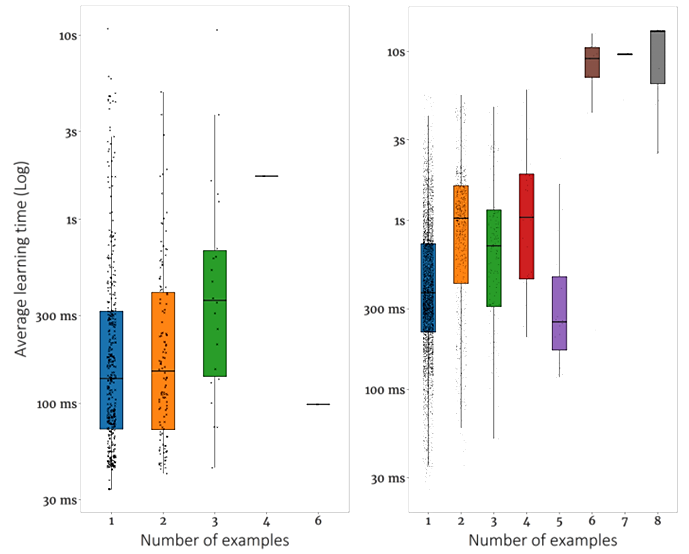
\includegraphics[width=\textwidth]{figures/perf}};
        \begin{scope}[x={(img.south east)}, y={(img.north west)}]
            \node[inner sep=10pt, rounded corners, fill=Tan] at (0.3, 1) {FlashFill};
            \node[inner sep=10pt, rounded corners, fill=Tan] at (0.78, 1) {FlashExtract};
            \node[fill=white] at (0.3, 0.02) { Number of examples };
            \node[fill=white] at (0.78, 0.02) { Number of examples };
            \node[fill=white, rotate=90] at (0.03, 0.52) { Average learning time (Log) };
        \end{scope}
    \end{tikzpicture}
    \caption{Performance evaluation of the reimplementations of FlashFill~\cite{flashfill} and
    FlashExtract~\cite{flashextract} on top of the PROSE framework.
    Each dot shows average learning time per iteration on a given scenario.
    The scenarios are clustered by the number of examples (iterations) required to complete the task.
    \emph{Left:} 531 FlashFill scenarios.
    \emph{Right:} 6464 FlashExtract scenarios.}
    \label{fig:prose:evaluation:perf}
\end{figure}

\subsection{Experiments}
\label{sec:prose:evaluation:experiments}

\paragraph{Performance \& Number of examples}
\Cref{fig:prose:evaluation:perf} shows performance and the number of examples of our FlashFill and FlashExtract
reimplementations on top of the PROSE framework.
The overall performance is comparable to that of the original system, even though the implementations differ
drastically.
For example, the runtime of the original implementation of FlashExtract varies from 0.1 to 4 sec, with a median of 0.3
sec~\cite{flashextract}.
The new implementation (despite being more expressive and built on a general framework) has a runtime of
$0.5-3$x the original implementation, with a median of 0.6 sec.
This performance is sufficient for the PROSE-based implementation to be successfully used in industry instead of the
original one.

\paragraph{VSA Volume}
There is no good theoretical bound on the time of VSA clustering (the most time-consuming operation in the deductive
search).
However, it is evident that the output VSA volume is proportional to the clustering time.
Thus, to evaluate it, we measured the VSA volume on our real-life benchmark suite.
As \Cref{fig:prose:evaluation:volume} shows, even for large inputs it never exceeds $8000$ nodes (thus explaining
efficient runtime), whereas VSA size (i.e. number of learned programs) may approach $10^{13}$.

\begin{figure}[t]
    \centering
    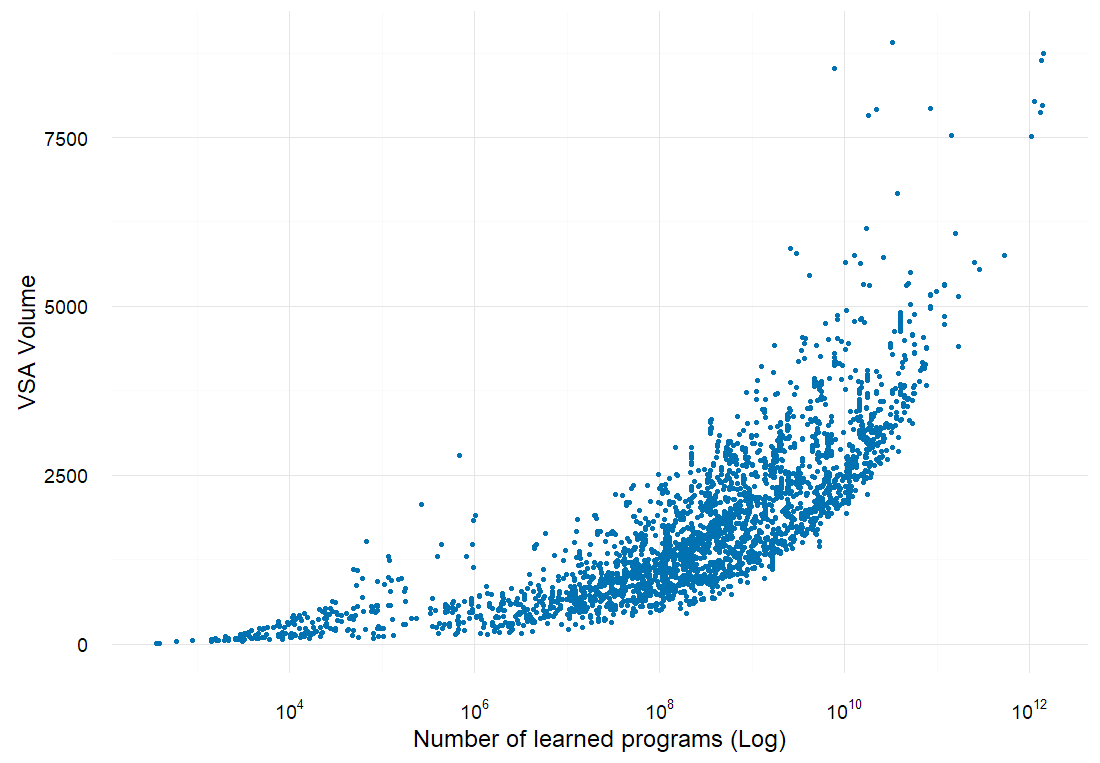
\includegraphics[width=1.0\linewidth]{figures/vsa-volume}
    \uwsinglespace
    \caption{The relationship between VSA volume and VSA size (i.e. number of programs) for the complete VSAs learned to
    solve 6464 real-life FlashExtract scenarios.}
    \label{fig:prose:evaluation:volume}
\end{figure}

\section{Strengths and Limitations}
\label{sec:prose:discussion}
The methodology of deductive search that lies at the core of PROSE works best under the following conditions:

\paragraph{Decidability}
A majority of the DSL should be characterized by witness functions, capturing a subset of inverse semantics of the DSL
operators.

An example of an operator that cannot be characterized by any witness function is an integral multivariate polynomial
$\mathsf{Poly}(a_0, \dots, a_k, X_1, \dots, X_n)$.
Here $a_0, \dots, a_k$ are integer polynomial coefficients, which are input variables in the DSL,
and $X_1, \dots, X_n$ are integer nonterminals in the DSL.
Given a specification $\spec = (a_0, \dots, a_k) \tospec y$ stating that a specific $\mathsf{Poly}$ executed with
coefficients $a_0, \dots, a_k$ evaluated to $y$ on \emph{some} $X_1, \dots, X_n$, a witness function~$\omega_j$ has to
find a set of possible values for $X_j$.
This requires finding roots of a multivariate integral polynomial, which is undecidable.

\paragraph{Deduction}
Witness functions should not introduce many disjunctions.
Each disjunct (assuming it can be materialized by at least one program) starts a new deduction branch.
In certain domains this problem can only be efficiently solved with a corresponding SMT solver.

Consider the bitwise operator $\mathsf{BitOr}\colon (\mathsf{Bit32}, \mathsf{Bit32}) \to \mathsf{Bit32}$.
Given a specification $\state \tospec b$ where $b\colon \mathsf{Bit32}$, witness functions for $\mathsf{BitOr}$
have to construct each possible pair of bitvectors $\langle b_1, b_2\rangle$ such that $\mathsf{BitOr}(b_1, b_2) = b$.
If $b = 2^{32} - 1$, there exist $3^{32}$ such pairs.
A deduction over $3^{32}$ branches is infeasible.

\paragraph{Performance}
Witness functions should be efficient, preferably polynomial in low degrees over the specification size.

Consider the multiplication operator $\mathsf{Mul}\colon (\mathsf{Int}, \mathsf{Int}) \to \mathsf{Int}$.
Given a specification $\state \tospec n$ with a multiplication result, a witness function for $\mathsf{Mul}$
has to factor $n$.
This problem is decidable, and the number of possible results is at most $\mathcal{O}(\log n)$, but the factoring itself
is infeasible for large $n$.

\paragraph{}
\indent All counterexamples above feature real-life operators, which commonly arise in embedded systems, control theory,
and other domains.
The best known synthesis strategies for them are based on specialized SMT solvers~\cite{sygus}.
On the other hand, to our knowledge PROSE is the \emph{only} synthesis strategy when the following (also real-life)
conditions hold:
\begin{itemize}[nosep]
    \item The programs may contain domain-specific constants.
    \item The DSL contains arbitrary executable operators that manipulate domain-specific objects with rich semantics.
    \item The specifications are inherently ambiguous, and resolving user's intent requires learning a set of valid
        programs to enable ranking or additional user interaction.
    \item The engineering and maintenance cost of a PBE\hyp{}based tool is limited by industrial budget and available
        developers.
\end{itemize}


